\documentclass[10pt,letter,notitlepage]{article}
%Mise en page
\usepackage[left=2cm, right=2cm, lines=45, top=0.8in, bottom=0.7in]{geometry}
\usepackage{fancyhdr}
\usepackage{fancybox}
\usepackage{pdfpages} 
\renewcommand{\headrulewidth}{1.5pt}
\renewcommand{\footrulewidth}{1.5pt}
\pagestyle{fancy}
\newcommand\Loadedframemethod{TikZ}
\usepackage[framemethod=\Loadedframemethod]{mdframed}
\usepackage{tikz}
\usepackage[linesnumbered,ruled,vlined]{algorithm2e}
%\usepackage{url}
\usepackage{dsfont}
\usepackage{amssymb,amsmath}
\usepackage{xspace}
\usepackage{graphicx} %插入图片的宏包
\usepackage{float} %设置图片浮动位置的宏包
\usepackage{subfigure} %插入多图时用子图显示的宏包
\usepackage{tabu}

\lhead{
\textbf{University of Waterloo}
}
\rhead{\textbf{2022 Spring}
}
\chead{\textbf{
CS480/680
 }}

\newcommand{\RR}{\mathds{R}}
\newcommand{\sign}{\mathop{\mathrm{sign}}}
\newcommand{\argmin}{\mathop{\mathrm{argmin}}}
\newcommand{\zero}{\mathbf{0}}
\newcommand{\one}{\mathbf{1}}
\newcommand{\bv}{\mathbf{b}}
\newcommand{\wv}{\mathbf{w}}
\newcommand{\xv}{\mathbf{x}}
\newcommand{\yv}{\mathbf{y}}
\newcommand{\rv}{\mathbf{r}}
\newcommand{\inner}[2]{\langle #1, #2 \rangle}
\newcommand{\red}[1]{{\color{red}#1}}
\newcommand{\blue}[1]{{\color{blue}#1}}
\newcommand{\magenta}[1]{{\color{magenta}#1}}


\newcommand{\ea}{{et al.}\xspace}
\newcommand{\eg}{{e.g.}\xspace}
\newcommand{\ie}{{i.e.}\xspace}
\newcommand{\iid}{{i.i.d.}\xspace}
\newcommand{\cf}{{cf.}\xspace}
\newcommand{\wrt}{{w.r.t.}\xspace}
\newcommand{\aka}{{a.k.a.}\xspace}
\newcommand{\etc}{{etc.}\xspace}

\newcommand{\ans}[1]{{\color{orange}\textsf{Ans}: #1}}


\lfoot{}
\cfoot{\textbf{Gautam Kamath (gckamath@uwaterloo.ca) \textcopyright 2022}}

%================================
%================================

\setlength{\parskip}{1cm}
\setlength{\parindent}{1cm}
\tikzstyle{titregris} =
[draw=gray,fill=white, shading = exersicetitle, %
text=gray, rectangle, rounded corners, right,minimum height=.3cm]
\pgfdeclarehorizontalshading{exersicebackground}{100bp}
{color(0bp)=(green!40); color(100bp)=(black!5)}
\pgfdeclarehorizontalshading{exersicetitle}{100bp}
{color(0bp)=(red!40);color(100bp)=(black!5)}
\newcounter{exercise}
\renewcommand*\theexercise{exercice \textbf{Exercice}~n\arabic{exercise}}
\makeatletter
\def\mdf@@exercisepoints{}%new mdframed key:
\define@key{mdf}{exercisepoints}{%
\def\mdf@@exercisepoints{#1}
}

\mdfdefinestyle{exercisestyle}{%
outerlinewidth=1em,outerlinecolor=white,%
leftmargin=-1em,rightmargin=-1em,%
middlelinewidth=0.5pt,roundcorner=3pt,linecolor=black,
apptotikzsetting={\tikzset{mdfbackground/.append style ={%
shading = exersicebackground}}},
innertopmargin=0.1\baselineskip,
skipabove={\dimexpr0.1\baselineskip+0\topskip\relax},
skipbelow={-0.1em},
needspace=0.5\baselineskip,
frametitlefont=\sffamily\bfseries,
settings={\global\stepcounter{exercise}},
singleextra={%
\node[titregris,xshift=0.5cm] at (P-|O) %
{~\mdf@frametitlefont{\theexercise}~};
\ifdefempty{\mdf@@exercisepoints}%
{}%
{\node[titregris,left,xshift=-1cm] at (P)%
{~\mdf@frametitlefont{\mdf@@exercisepoints points}~};}%
},
firstextra={%
\node[titregris,xshift=1cm] at (P-|O) %
{~\mdf@frametitlefont{\theexercise}~};
\ifdefempty{\mdf@@exercisepoints}%
{}%
{\node[titregris,left,xshift=-1cm] at (P)%
{~\mdf@frametitlefont{\mdf@@exercisepoints points}~};}%
},
}
\makeatother


%%%%%%%%%

%%%%%%%%%%%%%%%
\mdfdefinestyle{theoremstyle}{%
outerlinewidth=0.01em,linecolor=black,middlelinewidth=0.5pt,%
frametitlerule=true,roundcorner=2pt,%
apptotikzsetting={\tikzset{mfframetitlebackground/.append style={%
shade,left color=white, right color=blue!20}}},
frametitlerulecolor=black,innertopmargin=1\baselineskip,%green!60,
innerbottommargin=0.5\baselineskip,
frametitlerulewidth=0.1pt,
innertopmargin=0.7\topskip,skipabove={\dimexpr0.2\baselineskip+0.1\topskip\relax},
frametitleaboveskip=1pt,
frametitlebelowskip=1pt
}
\setlength{\parskip}{0mm}
\setlength{\parindent}{10mm}
\mdtheorem[style=theoremstyle]{exercise}{\textbf{Exercise}}

%================Liste definition--numList-and alphList=============
\newcounter{alphListCounter}
\newenvironment
{alphList}
{\begin{list}
{\alph{alphListCounter})}
{\usecounter{alphListCounter}
\setlength{\rightmargin}{0cm}
\setlength{\leftmargin}{0.5cm}
\setlength{\itemsep}{0.2cm}
\setlength{\partopsep}{0cm}
\setlength{\parsep}{0cm}}
}
{\end{list}}
\newcounter{numListCounter}
\newenvironment
{numList}
{\begin{list}
{\arabic{numListCounter})}
{\usecounter{numListCounter}
\setlength{\rightmargin}{0cm}
\setlength{\leftmargin}{0.5cm}
\setlength{\itemsep}{0cm}
\setlength{\partopsep}{0cm}
\setlength{\parsep}{0cm}}
}
{\end{list}}

\usepackage[breaklinks=true,letterpaper=true,linkcolor=magenta,urlcolor=magenta,citecolor=black]{hyperref}

\usepackage{cleveref}


%===========================================================
\begin{document}

\begin{center}
  \large{\textbf{CS480/680: Introduction to Machine Learning} \\ Homework 1\\ \red{Due: 11:59 pm, May 25, 2022}, submit on LEARN and/or Crowdmark (TBD).} \\

Name: Yusu (Cosmo) Zhao, Student ID: 20761282

\end{center}

\begin{center}
Submit your writeup in pdf and all source code in a zip file (with proper documentation). Write a script for each programming exercise so that the TAs can easily run and verify your results. Make sure your code runs!

[Text in square brackets are hints that can be ignored.]
\end{center}



\begin{exercise}[Perceptron Implementation (5 pts)]
\blue{\textbf{Convention:} All algebraic operations, when applied to a vector or matrix, are understood to be element-wise (unless otherwise stated).}
		
\begin{algorithm}[H]
\DontPrintSemicolon
	\KwIn{$X\in\RR^{n\times d}$, $\yv\in \{-1,1\}^n$, $\wv=\zero_d$, $b=0$, $\mathsf{max\_pass} \in \mathds{N}$}
	
	\KwOut{$\wv, b, mistake$}
	
	\For{$t=1, 2, \ldots, \mathsf{max\_pass}$ }{
		$mistake(t) \gets 0$
		
		\For{$i=1, 2, \ldots, n$}{
			\If{$y_i (\inner{\xv_i}{\wv}+b) \leq 0$}{
				$\wv \gets \wv + y_i\xv_i$ \tcp*{$\xv_i$ is the $i$-th row of $X$}
			
				$b \gets b + y_i$
			
				$mistake(t) \gets mistake(t) + 1$
			}	
		}
	}
	\caption{The perceptron algorithm.}
	\label{alg:perceptron}
\end{algorithm}
	
Implement the perceptron in \Cref{alg:perceptron}. Your implementation should take input as $X = [\xv_1^\top, \ldots, \xv_n^\top]^\top \in \RR^{n \times d}$, $\yv \in \{-1,1\}^{n}$, an initialization of the hyperplane parameters $\wv\in\RR^{d}$ and $b\in \RR$, and the maximum number of passes of the training set [suggested $\mathsf{max\_pass} = 500$]. Run your perceptron algorithm on the \href{https://archive.ics.uci.edu/ml/datasets/spambase}{\magenta{\textsf{spambase}}} dataset (use the version on the course website), and plot the number of mistakes ($y$-axis) \wrt the number of passes ($x$-axis).
		
\ans{	}

\begin{figure}[H]
\centering
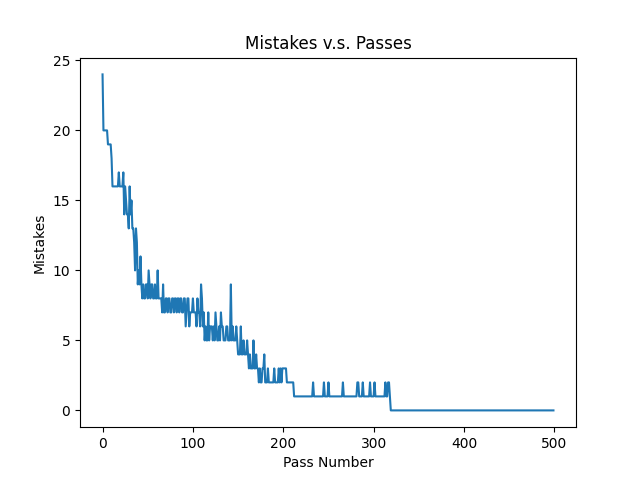
\includegraphics[width=0.7\textwidth]{Exercise1.png}
\caption{Mistakes v.s. Passes}
\label{Fig.main2}
\end{figure}

\end{exercise}


\begin{exercise}[Regression Implementation (8 pts)]
Recall that ridge regression refers to
\begin{align}
  \min_{\wv\in \RR^d, b\in \RR} ~ \overbrace{\underbrace{\tfrac{1}{2n} \|X \wv+ b\one - \yv\|_2^2}_{\mbox{error}} + \lambda \|\wv\|_2^2}^{\mbox{loss}}, \label{eq:regression}
\end{align}
where $X \in \RR^{n \times d}$ and $\yv \in \RR^n$ are the given dataset and $\lambda \geq 0$ is the regularization hyperparameter.
If $\lambda = 0$, then this is the standard linear regression problem.
  Observe the distinction between the error (which does not include the regularization term) and the loss (which does).

\begin{enumerate}
  \item (1 pt) Show that ridge regression can be rewritten as a non-regularized linear regression problem.
  That is, prove \ref{eq:regression} is equivalent to 
\begin{align}
  \min_{\wv\in \RR^d, b\in \RR} ~ \tfrac{1}{2n} \left\|\begin{bmatrix}
X & \one_n \\
    \sqrt{2\lambda n}I_d & \zero_d
    \end{bmatrix} \begin{bmatrix} \wv  \\ b\end{bmatrix}  - \begin{bmatrix}\yv \\ \zero_d\end{bmatrix}\right\|_2^2 , 
\end{align}
where $I_d$ is the $d$-dimensional identity matrix, and $\zero_k$ and $\one_k$ are zero and one column vectors in $k$ dimensions.
    
    \ans{
      \color{orange}
      We will prove that the two expressions are equal
      \begin{align*}
          \tfrac{1}{2n} \left\|\begin{bmatrix}
          X & \one_n \\
          \sqrt{2\lambda n}I_d & \zero_d
          \end{bmatrix} \begin{bmatrix} \wv  \\ b\end{bmatrix}  - \begin{bmatrix}\yv \\ \zero_d\end{bmatrix}\right\|_2^2 
          &= 
          \tfrac{1}{2n} \left\|\begin{bmatrix}
          X\wv + \one_nb \\
          \sqrt{2\lambda n}I_d\wv + \zero_db
          \end{bmatrix} - \begin{bmatrix}\yv \\ \zero_d\end{bmatrix}\right\|_2^2 \\
          &=
          \tfrac{1}{2n} \left\|\begin{bmatrix}
          X\wv + b\one_n - \yv\\
          \sqrt{2\lambda n}\wv
          \end{bmatrix}\right\|_2^2 \\
          &=
          \tfrac{1}{2n} \left(\sum_{i=1}^n (X_i\wv + b - \yv_i)^2 + \sum_{i=1}^d (\sqrt{2\lambda n}\wv_i)^2 \right) \\
          &=
          \tfrac{1}{2n} \left(\sum_{i=1}^n (X_i\wv + b - \yv_i)^2 + 2\lambda n\sum_{i=1}^d \wv_i^2 \right) \\
          &=
          \tfrac{1}{2n} \sum_{i=1}^n (X_i\wv + b - \yv_i)^2 + \lambda \sum_{i=1}^d \wv_i^2 \\
          &=
          \tfrac{1}{2n} \|X \wv+ b\one_n - \yv\|_2^2 + \lambda \|\wv\|_2^2
      \end{align*}
      From above, we proved that:
      $$
        \tfrac{1}{2n} \left\|\begin{bmatrix}
        X & \one_n \\
        \sqrt{2\lambda n}I_d & \zero_d
        \end{bmatrix} \begin{bmatrix} \wv  \\ b\end{bmatrix}  - \begin{bmatrix}\yv \\ \zero_d\end{bmatrix}\right\|_2^2 
        =
        \tfrac{1}{2n} \|X \wv+ b\one_n - \yv\|_2^2 + \lambda \|\wv\|_2^2
      $$
      so the minimum of them are equal, and (1) and (2) are equal.
    }

\item (1 pt) Show that the derivatives of \ref{eq:regression} are
\begin{align}
\frac{\partial}{\partial\wv} &=  \tfrac1n X^\top (X\wv + b\one - \yv) + 2 \lambda \wv\\
\label{eq:b}
\frac{\partial}{\partial b} &= \tfrac1n \one^\top (X\wv + b\one - \yv).
\end{align}

    \ans{
      From question 2, we know that:
      $$
        \tfrac{1}{2n} \|X \wv+ b\one_n - \yv\|_2^2 + \lambda \|\wv\|_2^2
        =
        \tfrac{1}{2n} \sum_{i=1}^n (X_i\wv + b - \yv_i)^2 + \lambda \sum_{i=1}^d \wv_i^2 \\
      $$
      \color{orange}
      So we have:
      \begin{align*}
        \frac{\partial}{\partial\wv} (1)&= \frac{\partial}{\partial\wv} \left(\tfrac{1}{2n} \sum_{i=1}^n (X_i\wv + b - \yv_i)^2 + \lambda \sum_{i=1}^d \wv_i^2\right) \\
        &= \begin{bmatrix} \frac{\partial}{\partial\wv_0} & \frac{\partial}{\partial\wv_1} & \cdots \end{bmatrix}^T
      \end{align*}
      For each $\wv_k$ for $k$ from $1$ to $d$:
      \begin{align*}
        \frac{\partial}{\partial\wv_j} (1)&= \frac{\partial}{\partial\wv_j} \left(\tfrac{1}{2n} \sum_{i=1}^n (X_i\wv + b - \yv_i)^2 + \lambda \sum_{i=1}^d \wv_i^2\right) \\
        &=
        \tfrac{1}{2n} \sum_{i=1}^n \left(\frac{\partial}{\partial\wv_j} (\sum_{k=1}^d X_{ik}\wv_k + b - \yv_i)^2\right) +
        \lambda \frac{\partial}{\partial\wv_j} \left(\sum_{i=1}^d \wv_i^2\right) \\
        &= 
        \tfrac{1}{n} \sum_{i=1}^n \left(\frac{\partial}{\partial\wv_j} \sum_{k=1}^d X_{ik}\wv_k\right)\left(\sum_{k=1}^d X_{ik}\wv_k + b - \yv_i\right) + 
        2\lambda \wv_j \\
        &=
        \tfrac{1}{n} \sum_{i=1}^n X_{ij}\left(\sum_{k=1}^d X_{ik}\wv_k + b - \yv_i\right) + 
        2\lambda \wv_j \\
        &= \tfrac{1}{n} \sum_{k=1}^d \sum_{i=1}^n X_{ij}X_{ik}\wv_k + \sum_{i=1}^nX_{ij}(b - \yv_i) + 2\lambda \wv_j \\
        &= \tfrac{1}{n}X^T_jX\wv+X^T_j(b\one_n-y) + 2\lambda \wv_j
      \end{align*}
      Therefore: 
      $$\frac{\partial}{\partial\wv} = \tfrac1n X^\top (X\wv + b\one - \yv) + 2 \lambda \wv$$
      Similarly:
      \begin{align*}
        \frac{\partial}{\partial b} &= \frac{\partial}{\partial b} \left(\tfrac{1}{2n} \|X \wv+ b\one_n - \yv\|_2^2 + \lambda \|\wv\|_2^2\right) \\.
        &= 2 \tfrac{1}{2n} \one_n^T(X \wv+ \one_nb - \yv)\\
        &= \tfrac1n \one^\top (X\wv + b\one - \yv)
      \end{align*}
      Because we can simple substitute $\one$ to $X$ above as these two equations have the same form, and do not depend on the matrix dimensions. 
    } 

  \item (2 pts) Implement ridge regression using the closed form solution for linear regression as derived in lecture. 
    You may find the function \texttt{numpy.linalg.solve} useful.

    \ans{From question 1 we know that: 
      $$
        \tfrac{1}{2n} \left\|\begin{bmatrix}
        X & \one_n \\
        \sqrt{2\lambda n}I_d & \zero_d
        \end{bmatrix} \begin{bmatrix} \wv  \\ b\end{bmatrix}  - \begin{bmatrix}\yv \\ \zero_d\end{bmatrix}\right\|_2^2 
        =
        \tfrac{1}{2n} \|X \wv+ b\one_n - \yv\|_2^2 + \lambda \|\wv\|_2^2
      $$
      So their gradients are also equal. By inspenction, we found that the left side has the form of $\|A'w'-z'\|_2^2$ with:
      $$
        A' = \begin{bmatrix}
        X & \one_n \\
        \sqrt{2\lambda n}I_d & \zero_d
        \end{bmatrix},
        w' = \begin{bmatrix} \wv  \\ b\end{bmatrix},
        z' = \begin{bmatrix}\yv \\ \zero_d\end{bmatrix}
      $$
      By the formula we introduce in lecture, we can find that the gradient is:
      $$
        \tfrac{1}{2n} (2A'^TA'w'-2A'^Tz')
      $$
      Setting the above gradient to zero, we get the equation:
      $$
        A'^TA'w'=A'^Tz'
      $$
      \color{orange}
      which is equivalent to:
      $$
        \begin{bmatrix}
        X & \one_n \\
        \sqrt{2\lambda n}I_d & \zero_d
        \end{bmatrix}^T
        \begin{bmatrix}
        X & \one_n \\
        \sqrt{2\lambda n}I_d & \zero_d
        \end{bmatrix}
        \begin{bmatrix} \wv  \\ b\end{bmatrix}
        = \begin{bmatrix}
        X & \one_n \\
        \sqrt{2\lambda n}I_d & \zero_d
        \end{bmatrix}^T\begin{bmatrix}\yv \\ \zero_d\end{bmatrix}
      $$
      }
\item (2 pts) Implement the gradient descent algorithm for solving ridge regression. The following \red{incomplete} pseudo-code may of help.
    Your training loss should monotonically decrease during iteration; if not try to tune your step size $\eta$, \eg make it smaller.

\begin{algorithm}[H]
\DontPrintSemicolon
	\KwIn{$X\in\RR^{n\times d}$, $\yv\in \RR^n$, $\wv_0=\zero_d$, $b_0=0$, $\mathsf{max\_pass} \in \mathds{N}$, $\eta > 0$, $\mathsf{tol} > 0$}

	\KwOut{$\wv, b$}

	\For{$t=1, 2, \ldots, \mathsf{max\_pass}$ }{
		$\wv_t \gets  $

		$b_t \gets $

		\If(\tcp*[f]{can use other stopping criteria}){$\|\wv_{t} - \wv_{t-1}\|  \leq \mathsf{tol}$}{
			\textbf{break}
		}
	}

	$\wv \gets \wv_t, ~ b \gets b_t$
	\caption{Gradient descent for ridge regression.}
	\label{alg:rr}
\end{algorithm}

    \ans{
      Notice that the multiplications below are mathmatical. They are not element-wise.
      $$
      \wv_t = \wv_{t-1} - \left(\tfrac{1}{n} X^\top (X\wv_{t-1} + b_{t-1}\one_n - \yv) + 2 \lambda \wv_{t-1}\right) *\eta
      $$

      $$
      b_t = b_{t-1} - \left(\tfrac{1}{n} \one_n^\top (X\wv_{t-1} + b_{t-1}\one_n - \yv)\right) *\eta
      $$
    }

  \item (3 pts) Test your two implementations on the Boston \href{http://lib.stat.cmu.edu/datasets/boston}{\textsf{\magenta{housing}}} dataset (to predict the median house price, \ie, $y$). 
    Use the train and test splits provided on course website. 
    Try $\lambda \in \{0, 10\}$ and report your training error, training loss and test error for each.
    \red{You may have trouble getting gradient descent to work if you don't \href{https://scikit-learn.org/stable/modules/preprocessing.html}{standardize} your data (you may not use sklearn to standardize your data, do it yourself).
    Note that you would have to standardize both your training and test features.
    (Try gradient descent both without and with standardizing the data and see how it differs.)}
    For the gradient descent algorithm, plot the training loss over iterations. 
    Compare the running time of the two approaches, which is faster?
    Overall, which approach do you think is better? Explain why.

    \ans{} \\
    {\color{orange}
    The graph is attached below. And the training error and test error are listed as follows: \\
    \begin{tabular}{|c|c|c|c|}
    \hline methods&train error&training loss&test error\\
    \hline lambda0, closed form&4.847149319454688&4.847149319454688&185.11147877100467 \\
    \hline lambda10, closed form&38.728489031407676&38.815542966133066&57.10971556808989 \\
    \hline lambda0, gradient descent&36.327071579707585&See Graph Below&47.71665235364033 \\
    \hline lambda10, gradient descent&44.607081689993855&See Graph Below&39.79430484819916 \\
    \hline
    \end{tabular}
    

    The running time of closed form is 0ms, while the running time
    for the gradient descent algorithm is about 0.0625 ms, or 62500000 ns, both are measured in CPU time. 
    So the closed form is definitely faster.
    Overall in this case, I think I would prefer the closed form solution. Firstly, it runs much faster.
    Secondly, the result generated by the two methods should be the same, since theoretically they will give 
    the same solution vector (both are looking for the minimum in convex functions). 
    The acutal test error are also close
    However, the closed form only works here because this is linear regression and we are able to derive it. 
    If we cannot even derive the form, then gradient descent will be the only option. 
    }
    \begin{figure}[H]
    \centering
    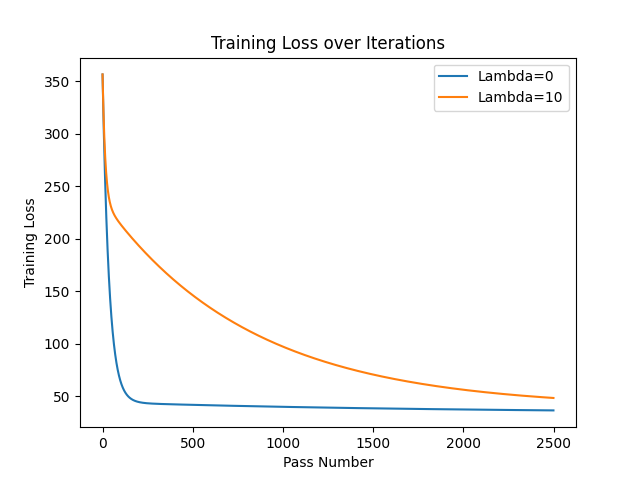
\includegraphics[width=0.7\textwidth]{Exercise2.png}
    \caption{Training Loss over Iterations}
    \label{Fig.main3}
    \end{figure}


\end{enumerate}
\end{exercise}

\begin{exercise}[Playing with Regression (3 pts)]

  \red{You may use the Python package scikit-learn for this exercise (and only for this exercise).}

Train (unregularized) linear regression, ridge regression, and lasso on the mystery datasets A, B, and C on the course website (using X\_train and Y\_train for each dataset).
For ridge regression and lasso, use k-fold cross validation to determine appropriate choices of the hyperparameters (you may NOT use functions like RidgeCV and LassoCV, you must implement it yourself). 
Report the average mean squared error on the test set for each method, as well as the selected regularization parameters.
Which approach performs best in each case?
For each dataset (A, B, C), do the following:
Create a histogram where the x-axis is divided into bins corresponding to the values of coordinates of the parameter vector, and the y-axis is the number of coordinates of the parameter vector which fall into each bin. 
Plot the three parameter vectors (one for unregularized, one for ridge, one for lasso) on the same histogram, so they're all visible at once (change the opacity setting for the bars if necessary).
  [There should be three total histograms, each with three parameter vectors overlayed.]

  \ans{
    \begin{figure}[H]
    \centering
    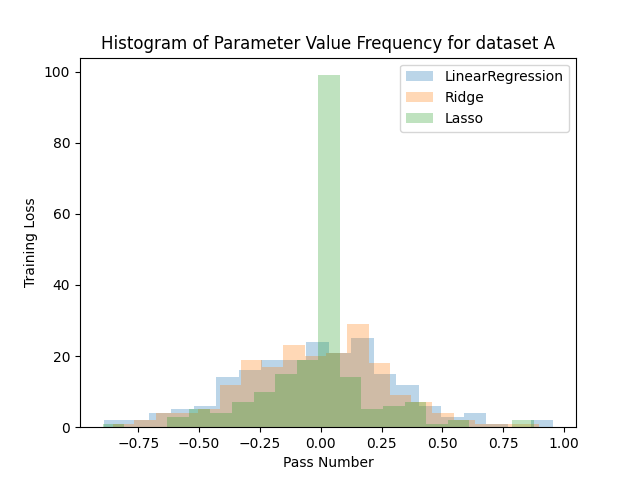
\includegraphics[width=0.7\textwidth]{Exercise3_dataset_A.png}
    \caption{Histogram of Parameter Value Frequency for dataset A}
    \end{figure}
    \\
    \color{orange}
    For dataset A:  \\
    Model: LinearRegression gives MSE = 3.247400173556322 \\
    Model: Ridge gives MSE = 2.77803413209245 with lambda = 10 \\
    Model: Lasso gives MSE = 6.1844343662602865 with lambda = 0.1 \\
    It seems like the best model is the ridge regression in this case since it gives the lowest MSE. \\

    \begin{figure}[H]
    \centering
    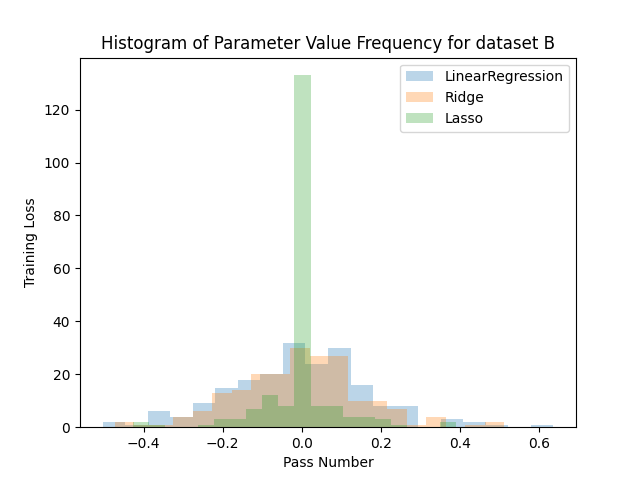
\includegraphics[width=0.7\textwidth]{Exercise3_dataset_B.png}
    \caption{Histogram of Parameter Value Frequency for dataset B}
    \end{figure}

    For dataset B: \\
    \color{orange}
    Model: LinearRegression gives mse = 2.7426823746517033 \\
    Model: Ridge gives mse = 2.059713219854696 with lambda = 10 \\
    Model: Lasso gives mse = 2.610022700635093 with lambda = 0.1 \\
    It seems like the best model is the ridge regression in this case since it gives the lowest MSE. But the difference
    among them are not significant\\
    \begin{figure}[H]
    \centering
    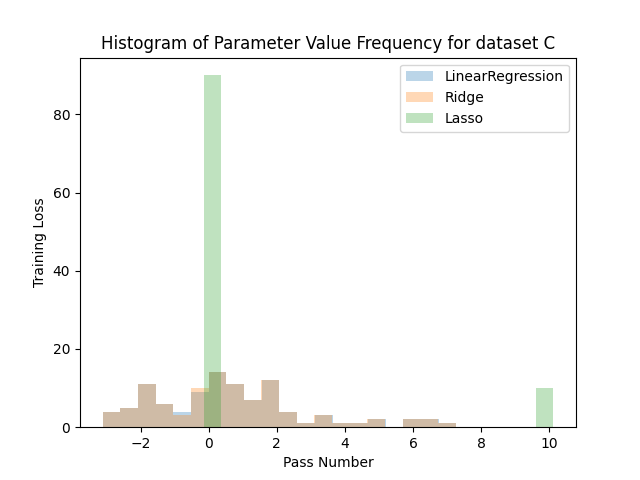
\includegraphics[width=0.7\textwidth]{Exercise3_dataset_C.png}
    \caption{Histogram of Parameter Value Frequency for dataset C}
    \end{figure}
    For dataset C: \\
    Model: LinearRegression gives mse = 506.1084477369717   \\
    Model: Ridge gives mse = 506.24141706882205 with lambda = 0.1 \\
    Model: Lasso gives mse = 1.2485953471555624 with lambda = 0.1 \\
    It seems like the best model is the lasso regression in this case since it gives the lowest MSE.\\
  }
\end{exercise}

\begin{exercise}[Nearest Neighbour Regression (7 pts)]
  \begin{enumerate}
    \item (3 pts) Implement $k$-nearest neighbour regression, for a dataset of $n$ $X, y$ pairs where $X \in \mathbb{R}^d$ and $y \in \mathbb{R}$. 
      This is similar to $k$-nearest neighbour classification, but instead of aggregating labels by taking the majority, we average the $y$ values of the $k$ nearest neighbours.
      Use $\ell_2$ distance as the distance metric, that is, the distance between points $X_1$ and $X_2$ is $\|X_1 - X_2\|_2$.
      Ensure that your implementation is $O(nd)$ time for all values of $k$, and argue that this is the case.

    \ans{

    \begin{algorithm}[H]
    \DontPrintSemicolon
      \KwIn{$X_{train}\in\RR^{n\times d}$, $\yv_{train}\in \RR^n$, $X \in \RR^d$, $k \in \mathds{N}$}
      
      \KwOut{$\yv_{new}$}
      
      \For{$t=1, 2, \ldots, n$ }{
        $dist(t) \gets dist(X, X_{train}[i])$
      }
        
      $kth = quickSelect(dist, 0, len(dists) - 1, k)$ \\
      $sum \gets 0$ \\
      \For{$i=1, 2, \ldots, n$}{
        \If{$dist(i) \leq kth$}{
          $sum \gets sum + \yv_{train}[i]$ 
        }	
      }
      $\yv_{new} \gets sum / k$
      \caption{The perceptron algorithm.}
    \end{algorithm}

      \color{orange}
      The code is in file q4.py. \\
      To calculate the distance, which is the L2-norm, it takes $O(d)$, since we need to iterate over the vector and 
      do $O(1)$ operation in each iteration. Then, we do it for each $X_{train}[i]$. So the L2-norm calculation takes $O(nd)$.\\
      Then, we do a quick selection to find the k-th smallest element in the distance. Quick select algorithm will take $O(n)$ in average. \\
      Finally, we loop through the $X$ again, and find out all elements that is less than or equal to the k-th element and add the 
      corresponding y to the sum. This only takes $O(n)$ time. 
      The retuning value of $y_{new}$ only takes $O(1)$. \\
      Overall, this algorithm will take $O(nd) + O(n) + O(n) + O(1) = O(nd)$ in average. 
    }
    \item (2 pts) For the training sets of the $d=1$ mystery datasets D and E on the course website, compute a) the (unregularized) least squares linear regression solution and b) the $k$-nearest neighbour regression solution with each integer $k$ from $1$ to $9$.
      For each dataset, on one plot with the $x$ and $y$ axes corresponding to the $x$ and $y$ values, display the least squares solution, the $1$-nearest neighbour solution, and the $9$-nearest neighbour solution. 
      Be sure to plot these solutions for all points between the minimum and maximum $x$ values, not just for the points in the dataset.
      On another plot, with $k$ on the $x$ axis and test mean-squared error on the $y$ axis, display the error of the $k$-NN solution for each value of $k$. 
      On the same plot, include the test error of the least squares solution as a horizontal line.
      When does each approach perform better, and why? 

    \ans{
      \begin{figure}[H]
      \centering
      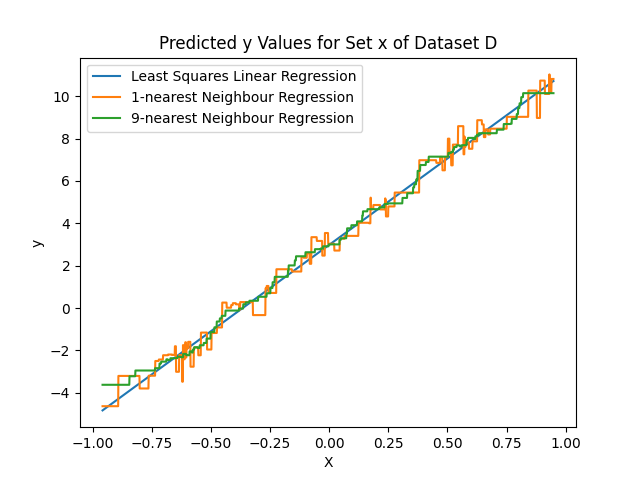
\includegraphics[width=0.7\textwidth]{Exercise4_dataset_D_all_points.png}
      \caption{Solutions for dataset D}
      \end{figure}

      \begin{figure}[H]
      \centering
      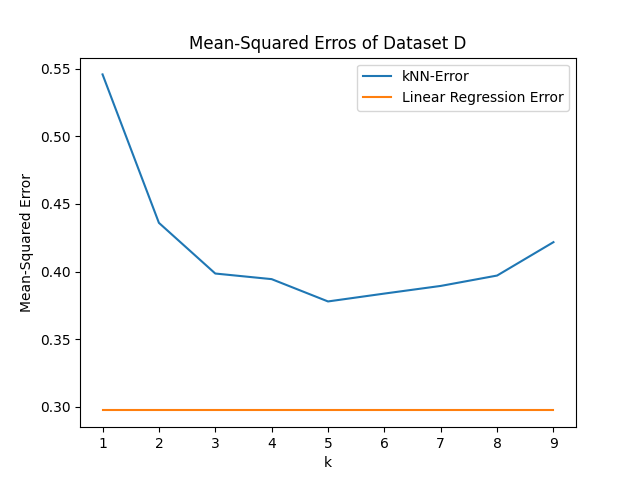
\includegraphics[width=0.7\textwidth]{Exercise4_dataset_D_error.png}
      \caption{Errors for dataset D}
      \end{figure}
      
      \color{orange}
      It looks like the linear regression is better for dataset D since it has a smaller mean squared error. \\
      If we look at how the datapoints, we can see that the datapoints are spread linearly, which is perfect for 
      linear regression to model it. 
      \begin{figure}[H]
      \centering
      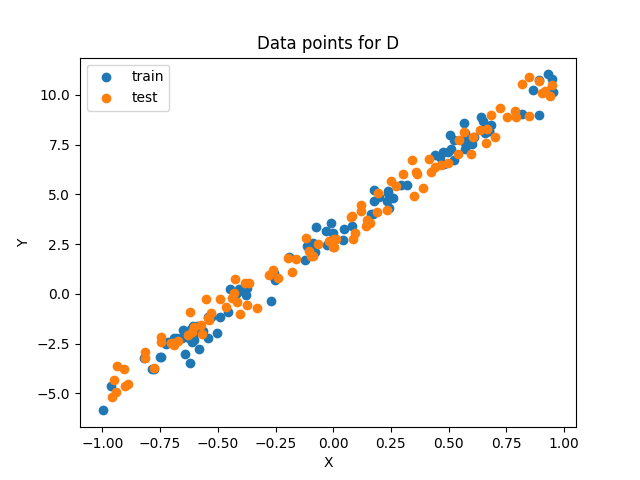
\includegraphics[width=0.7\textwidth]{Exercise4_dataset_D_datapoints.png}
      \caption{Datapoints for dataset D}
      \end{figure}


      \begin{figure}[H]
      \centering
      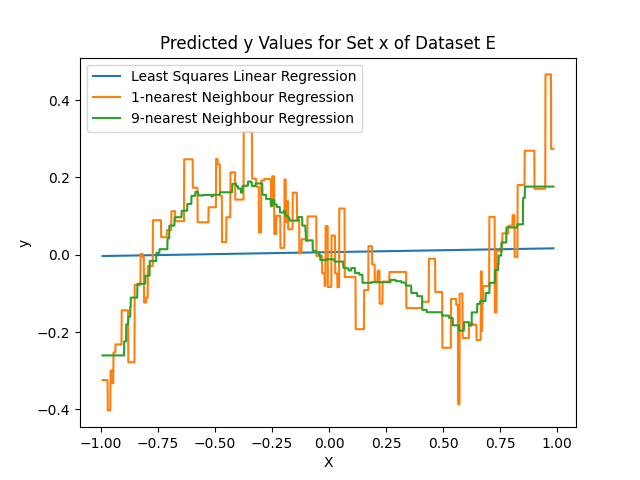
\includegraphics[width=0.7\textwidth]{Exercise4_dataset_E_all_points.png}
      \caption{Solutions for dataset E}
      \end{figure}

      \begin{figure}[H]
      \centering
      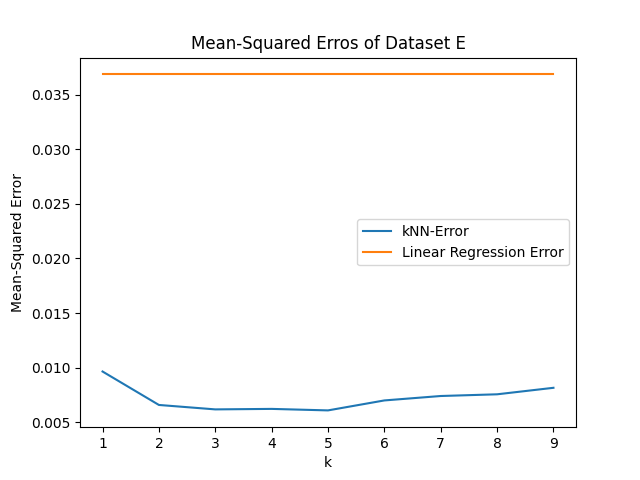
\includegraphics[width=0.7\textwidth]{Exercise4_dataset_E_error.png}
      \caption{Errors for dataset E}
      \end{figure}
      
      \color{orange}
      It looks like the k-nn regression is better for dataset E since it has a smaller mean squared error. 
      More specifically, the 5-NN is the best.
      In this case, our datapoints are pretty much like a sine wave, and linear regression cannot predict it 
      very well in this case. We can see from the solution diagram that the linear regression gives about a straigh line.
      The result is probably the best "linearly" fit of the data, but cannot be good for predicting the value, especially that 
      this is not a binarly classifier. Instead, the nearest neighbour algorithm can give result of the "sine wave" like 
      curve because it depends on the datapoints close to the point. In other words, in this dataset, the data points closer 
      to the actual point are more important. 
      \begin{figure}[H]
      \centering
      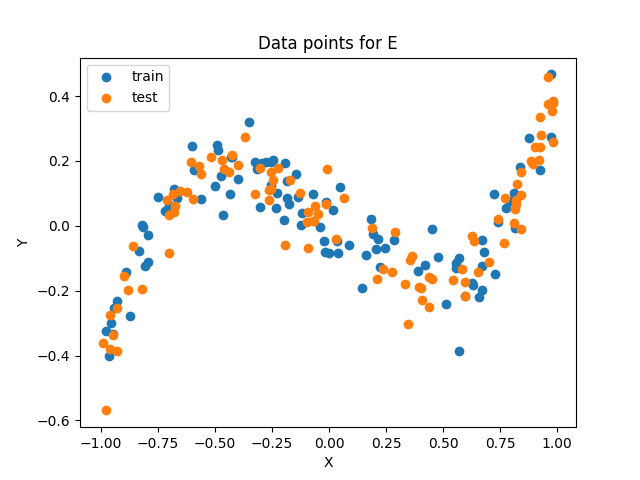
\includegraphics[width=0.7\textwidth]{Exercise4_dataset_E_datapoints.png}
      \caption{Datapoints for dataset E}
      \end{figure}
    }
    \item (2 pts) For the training set of the $d = 20$ mystery dataset F on the course website (\red{Dataset on course website updated May 15}), compute a) the (unregularized) least squares linear regression solution and b) the $k$-nearest neighbour regression solution with each integer $k$ from $1$ to $9$.
      Plot, with $k$ on the $x$ axis and test mean-squared error on the $y$ axis, display the error of the $k$-NN solution for each value of $k$. 
      On the same plot, include the test error of the least squares solution as a horizontal line.
      Which approach performs better, and why? 
      Hint: consider inspecting distances between the test points and their $k$ nearest neighbours in the training set.

    \ans{

      \begin{figure}[H]
      \centering
      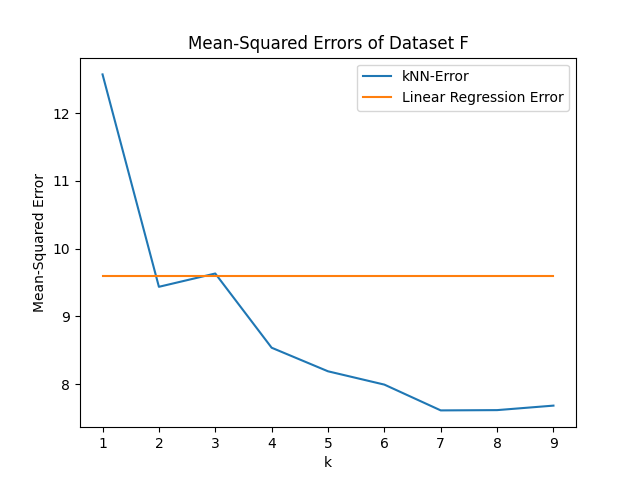
\includegraphics[width=0.7\textwidth]{Exercise4_dataset_F_error.png}
      \caption{Errors for dataset F}
      \end{figure}
      \color{orange}
      It looks like the k-nn regression is better for dataset F since it has a smaller mean squared error. 
      More specifically, the 7-NN is the best. \\
      A sample data of the distance between the test data point and the train data point is as follows: \\
      (2.739081206438655, 2.7819777208056644, 2.980837647067063, 3.0328653312547393, 3.053496114967776, 3.085910664335926, 3.1002830933648524,
      3.106419540372066, 3.17015836472704, 3.176246530582605, 3.24164282224411,\\
      3.262594462096352, 3.3044890637952613, 3.3055354256469833, 3.309942414538081, 3.3630879735638666, 3.3767138978681652) \\
      This is in sorted order. In fact, it looks like our test data point are almost about the same distance from 
      its neighbours. In this example, the test data point are around 3 unit far from its closest 50 neighbours.
      This means our test data points are about in the "center" of the train data set. In that case, the linear 
      regression model is probably not gonna help. Instead, if we use kNN with more neighbours and we use the 
      average as the aggregate function, then the result might be more correct. If we look at the mean square 
      graph, we can see that when we are using fewer neighbours, the error is huge, and that is likely because 
      the model is "biased". (The test data is in the "center" of other data points, but we only used one to model it).
      As we use more and more neighbours, we are getting closer and closer to the real value. 

    }
  \end{enumerate}
\end{exercise}

\end{document}
              
